\section{Decision criteria}
\label{sec:decision}

A common observation is that increasing the grid resolution or the polynomial degree of the basis functions will decrease the difference between the finite element approximation $u_\text{hp}$ and the actual solution $u$.

In fact, the impact of these adaptation techniques on this error is well understood. \textcite[Thm.~3.4]{babuska1990} determined an upper bound for the error that depends both on the cell diameter $h$ and the polynomial degree $p$:
\begin{align}
\label{eq:errorbound_hp} \left\|e_\text{hp}\right\|_{H^{1}(\Omega)} &\leq C \, h^{\mu} \, p^{-(m-1)} \, \|u\|_{H^{m}(\Omega)} \,\text{,}
\end{align}
where $e_{hp} = u - u_\text{hp}$ denotes the error function, $m$ is a measure for the regularity of the solution $u$, $C$ is a constant dependent on $m$, and $\mu = \min \left(p, m - 1\right)$.

These modifications do not have to happen uniformly on a global scale, but can be applied locally, since the global error consists of the local ones of each cell $K$:
\begin{align}
\label{eq:error_sum} \left\|e_\text{hp}\right\|_{H^1(\Omega)}^2 = \sum\limits_{K \in \Omega} \left\|e_\text{hp}\right\|_{H^1(K)}^2 \,\text{.}
\end{align}
Thus it all comes down to find those sections that have a significant contribution to the global error, and mitigate their impact by local adaptation.

On a reasonable family of quasiuniform meshes with an identical polynomial degree of all finite elements, \textcite[Sec.~1]{babuska1996} found the following upper bounds for the global error relative to the number of \glspl{dof} $n_\text{dofs}$ if the solution $u$ is sufficiently regular:
\begin{align}
\label{eq:errorbound_ana} \left\|e_\text{hp}\right\|_{H^{1}(\Omega)} &\leq C \, n_\text{dofs}^{- p/\text{dim}} \,\text{,} \\
\left\|e_\text{hp}\right\|_{H^{1}(\Omega)} &\leq C \, \exp\left(- b \, n_\text{dofs}^{1/\text{dim}} \right) \,\text{,}
\end{align}
where constants $b > 0$ and $C$ are both dependent on $m$, but independent of $n_\text{dofs}$.
%The first equation corresponds to the case that an upper bound for the polynomial degree of all used finite elements exists, while the second one omits this requirement.
On suitably chosen \hp-adaptive meshes however, \textcites[Thm.~5.1]{guo1986}[Thm.~2.5.2, Thm.~3.5.1]{babuska1996} predicted an even stronger exponential convergence for elliptic problems under the assumption that the solution $u$ is sufficiently regular:
\begin{align}
\label{eq:errorbound_exp} \left\|e_\text{hp}\right\|_{H^{1}(\Omega)} &\leq C \, \exp\left(- b \, n_\text{dofs}^\alpha \right) \,\text{,}
\end{align}
where constants $b > 0$ and $C$ are both independent of $n_\text{dofs}$, and $\alpha = 1/3$ for two or $\alpha = 1/5$ for three dimensional problems.

With sufficient information about the investigated scenario, an \hp-adaptive grid can be tailored to its specifics manually. However, grid adjustments by hand may not be optimal. Furthermore, not all peculiarities about the scenario are generally known in advance, which is especially the case for problems with complex geometries and time dependent ones.

Hence we need to elaborate on algorithms to automatically decide which subsets of the domain qualify for adaptation. With this technique, we typically set up a coarse mesh along with basis functions of a low polynomial degree and obtain a tailored mesh after several adaptation iterations.

In this section, we present different ways to identify areas whose adaptation will be most profitable, and to choose the most beneficial type of adaptation. For \hp-adaptation in particular, \textcite{mitchell2014} reviewed and compared a selection of strategies in detail. We demonstrate a subset of their recommendations in terms of performance and applicability, i.e.\@ those strategies that only require locally relevant part of the current solution.



\subsection{Adaptation strategies}
\label{ssec:strategy}

We will decide on the basis of adaptation criteria on each individual cell whether it will be considered for adaptation. Typical criteria involve comparing errors or their estimates to some absolute or relative threshold. Alternatively, also predicted errors or smoothness indicators are used for this purpose, as presented in the following sections. \textcite[Sec.~5.2]{bangerth2003} describe non-trivial strategies on how to decide based on these adaptation criteria, from which we present a commonly used selection.

So called \textit{fixed-error-reduction} or \textit{fixed-fraction} strategies select subsets of cells whose criteria accumulate to a predefined fraction of their global sum. This strategy is only applicable when the sum of all criteria actually has meaning, for example local errors which add up to the global one. Further, it may lead to optimal meshes for several problems, but tends to only adapt very few cells whenever singularities are encountered.

On the other hand, strategies known as \textit{fixed-rate} or \textit{fixed-number} pick predefined fractions of cells with the lowest or highest criteria for adaptation. This allows to predict the growth of cells, but may not lead to an optimal mesh since more cells may be adapted than necessary. We will use this strategy in our investigations presented in Ch.~\ref{ch:results}.

For either strategy, when using actual errors or error indicators as adaptation criteria, we typically select the subset of cells corresponding to the higher error for refinement, while the subset with the lower error is considered for coarsening.

Applicable implementations of these strategies involve binary searches to determine the section of cells relevant for adaptation. For parallel computations, according algorithms have been developed by \textcites[Sec.~3.1]{burstedde2008}[Sec.~5.1]{bangerth2012}.



\subsection{Error estimation}
\label{ssec:estimation}

The determination of the error for our finite element approximation requires the actual solution to be at our disposal. However, this is not the case in general, and we need to come up with an alternative measure.

\textcite{kelly1983} worked out an \textit{a posteriori} error estimator for the generalized Poisson equation $-\nabla \cdot \left( a \nabla u \right) = f$, where $a$ is a function usually describing material characteristics. They determined an upper bound $\eta_K$ for the error on each cell by balancing the gradient of the finite element approximation $u_\text{hp}$ on all faces $F$ of the cell's boundary:
\begin{align}
\label{eq:kelly} \|e_\text{hp}\|_{H_1(\Omega)}^2 &\leq C \sum\limits_{K \in \Omega} \eta_K^2 &&\text{with}&  \eta_K^2 &= \sum\limits_{F \in \partial K} c_F \int\limits_{F} \left[ a \, \frac{\partial u_\text{hp}}{\partial n} \right]^2 \differential{o} \,\text{,}
\end{align}
where $C$ is independent of the solution, but depends on $a$, and
\begin{align*}
\left[ a \, \frac{\partial u_\text{hp}}{\partial n} \right] = \left. a \, \frac{\partial u_\text{hp}}{\partial n_K} \right|_K + \left. a \, \frac{\partial u_\text{hp}}{\partial n_J}\right|_J
\end{align*}
denotes the jump of the approximation's gradient on the face between two adjacent cells $K$ and $J$. Hence \textcite{ainsworth1997a} attribute this estimator to the class of gradient recovery estimators.

The constant $c_F$ depends on the characteristics of each individual face of the cell. \textcite{kelly1983} originally used the constant $c_F = \frac{h_K}{24 \, a_\text{min} \, p_K}$ on each face, on which we determine the minimum $a_\text{min}$ of the given function. Here, $h_K$ and $p_K$ denote both cell diameter and polynomial degree of the finite element on cell $K$, respectively. \textcite{davydov2017} proposed a different constant for \hp-adaptive \gls{fem}: They recommend $c_F = \frac{h_F}{2 \, a_\text{min} \, p_F}$ with $h_F$ the face diagonal and $p_F = \max\left(p_K, p_J\right)$ the largest polynomial degree of adjacent elements $K$ and $J$ on this particular face.

This estimator has been worked out for the Poisson equation, but has proven its applicability on other problems as well, where this is no longer meant to be an estimator, but rather an error indicator \cite{dealiikelly}.

We will use these error estimates to decide which cells we will adapt. We are still left to decide which type of adaptation we want to apply, i.e.\@ \h-adaptation or \p-adaptation.



\subsection{Error prediction}
\label{ssec:prediction}

\cite{babuska1990} determined upper error bounds for numerical solutions based the distribution of finite elements. Both mesh resolution and polynomial degrees of the basis functions have a different, yet quantifiable influence on the error leading to Eq.~(\ref{eq:errorbound_hp}).

Their findings are valid not only for the numerical solution on a global scope, but on subsets of the domain as well. Local changes by \h- and \p-adaptation will thus result in different local error bounds. This motivates a strategy to locally decide which type of adaptation to impose based on the refinement history which has been proposed by \textcite{melenk2001}: We can predict how the current error will change whenever certain areas of our domain are considered for adaptation in the following iteration. These predicted error estimates allow us to decide whether the choice of adaptation in the previous step was justified, and provide the foundation for it on the next one.

We determine how the error bounds on two different distributions of finite elements will change by calculating their ratio. For this, we assume that both the actual error and its upper bound change with the same rate, which allows us to equate both ratios. We further assume that the solution is sufficiently regular ($m \gg p$). The ratio of errors then reads:
\begin{align}
\label{eq:errorratio_hp} \frac{\left\|e_{h_\text{f} p_\text{f}}\right\|_{H^{1}(\Omega)}}{\left\|e_{h_\text{a} p_\text{a}}\right\|_{H^{1}(\Omega)}} = \frac{h_\text{f}^{p_\text{f}}}{h_\text{a}^{p_\text{a}}} \, \left(\frac{p_\text{f}}{p_\text{a}}\right)^{-(m-1)} \,\text{,}
\end{align}
where subscripts $a$ and $f$ denote the finite element that is currently active or will be active after adaptation, respectively.

If we only consider \h-adaptation and leave the polynomial degree of the basis function unchanged ($p_\text{f} = p_\text{a} \equiv p$), we end up with the classical error bound \parencite{babuska1990}:
\begin{align}
\label{eq:errorratio_h} \frac{\left\|e_{h_\text{f} p}\right\|_{H^{1}(\Omega)}}{\left\|e_{h_\text{a} p}\right\|_{H^{1}(\Omega)}} = \left( \frac{h_\text{f}}{h_\text{a}} \right)^p \,\text{.}
\end{align}

However, if only \p-adaptation is considered and we keep the domain unchanged ($h_\text{f} = h_\text{a} \equiv h$), the ratio of errors still depends on the regularity of the actual solution which is not at our disposal in general. Following the considerations of \cite{melenk2001}, we expect \p-adaptation to change the error exponentially with the increment of the polynomial degree:
\begin{align}
\label{eq:errorratio_p} \frac{\left\|e_{h p_\text{f}}\right\|_{H^{1}(\Omega)}}{\left\|e_{h p_\text{a}}\right\|_{H^{1}(\Omega)}} = h^{p_\text{f} - p_\text{a}} \, \left(\frac{p_\text{f}}{p_\text{a}}\right)^{-(m-1)} \simeq c^{p_\text{f} - p_\text{a}} \,\text{,}
\end{align}
where $c$ is a constant independent of the cell diameter $h$.

We suggest a similar approach for the \hp-adaptation case as well. The above ratio assumes that the underlying mesh has not been changed. We thus identify Eq.~(\ref{eq:errorratio_p}) with an unaltered cell diameter ($h \equiv h_\text{a}$) in Eq.~(\ref{eq:errorratio_hp}) resulting in:
\begin{align}
\label{eq:errorratio_hp_exp} \frac{\left\|e_{h_\text{f} p_\text{f}}\right\|_{H^{1}(\Omega)}}{\left\|e_{h_\text{a} p_\text{a}}\right\|_{H^{1}(\Omega)}} \simeq \left( \frac{h_\text{f}}{h_\text{a}} \right)^{p_\text{f}} \, c^{p_\text{f} - p_\text{a}} \,\text{.}
\end{align}

Now, we will use these findings to develop an algorithm to predict errors of our finite element approximation. \textcite{melenk2001} worked out such an algorithm for \hp-refinement, which we will extend to \hp-coarsening as well. First, we will now only consider individual cells on our domain rather than the whole domain itself. Further, in practical applications, the actual error on these may be not at our disposal. Instead, we use suitable error indicators $\left\|e_{hp}\right\|_{H^{1}(K)} \simeq \eta_K$, assuming that they change with the same rate as the actual error.

We apply our consideration summarized in Eq.~(\ref{eq:errorratio_hp_exp}) on any form of adaptation. However, \h-adaptation poses an additional challenge, since we have to distribute errors from parent to children cells in case of refinement, or combine them in reverse for coarsening. Here, we will only consider isotropic \h-adaptation of quadrilaterals in two and hexahedrals in three dimensions, so that exactly $2^\text{dim}$ children are assigned to a cell, and the ratio of cell diameters $h_\text{f} / h_\text{a}$ is fixed to be $0.5$ for refinement and $2$ for coarsening. Further, the predicted error of a refined cell is distributed equally on all of its children, while the error of all coarsened cells is summed up for their parent. We assign future finite elements with their corresponding polynomial degrees on parent and children cells as described in Sec.~\ref{sec:adaptation}. Last, similar to \textcite{melenk2001}, we introduce control parameters $\gamma_n, \gamma_h \in (0, \infty)$, as well as $\gamma_p \in (0,1)$ for all three forms of adaptation, i.e.\@ no, \h-, and \p-adaptation. We end up with a set of equations which covers all possible combinations for \hp-adaptation:
\begin{align}
&\text{no adaptation:} & \eta^\text{pred}_K &= \eta_K \, \gamma_n \,\text{,} \\
&\text{\p-adaptation:} & \eta^\text{pred}_K &= \eta_K \, \gamma_p^{p_{\text{f},K} - p_{\text{a},K}} \,\text{,} \\
&\text{\hp-refinement:} &\eta^\text{pred}_{K_c} &= 0.5^{\text{dim}} \, \eta_{K_p} \, \gamma_h \, 0.5^{p_{\text{f},K_c}} \, \gamma_p^{p_{\text{f},K_c} - p_{\text{a},K_p}} \,\text{,} \\
&\text{\hp-coarsening:} & \eta^\text{pred}_{K_p} &= \sum\limits_{c} \eta_{K_c} \left( \gamma_h \, 0.5^{p_{\text{f},K_p}} \right)^{-1} \, \gamma_p^{p_{\text{f},K_p} - p_{\text{a},K_c}} \,\text{.} 
\end{align}
To clarify roles during \h-refinement and \h-coarsening, we marked parent cells $K_p$ and their children $K_c$ with corresponding subscripts, respectively.

We now have an algorithm to predict the error for the next adaptation step on basis of the current one. We are left to find a suitable criterion on how to use it to actually decide which type of adaptation to apply.

The original idea of \cite{melenk2001} was to compare the actual error of a cell $\eta_K$ in an adaptation cycle to its prediction $\eta_K^\text{pred}$ from the previous cycle. On all cells flagged for refinement, they consider \h-refinement for $\eta_K > \eta_K^\text{pred}$ and \p-refinement otherwise. We will extend these consideration to work for coarsening as well: For this, we need to pick the according strategy that keeps the cell diameter $h_k$ small for $\eta_K > \eta_K^\text{pred}$, and the polynomial degree $p_K$ large otherwise. The motivation behind this particular choice is that we keep the grid resolution fine whenever we suspect a singularity, which is usually indicated by a local error larger than its prediction.

An alternative approach would be to use the \textit{fixed-number} adaptation strategy from above: As indicators for each cell, we calculate the difference of predicted and estimated errors $(\eta_K^\text{pred} - \eta_K)$ for each subset of cells flagged for refinement and coarsening, respectively. On cells to be refined, we consider the fraction corresponding to the largest values for \p-adaptation, while for cells to be coarsened, the fraction with the lowest values will be picked. This conforms to the same argumentation as in the original variant. A graphical illustration of the assignment of cells for \hp-adaptation using this approach is given in Fig.~\ref{fig:indicators}. We will use this strategy in our applications presented in Ch.~\ref{ch:results}.

\begin{figure}
\centering
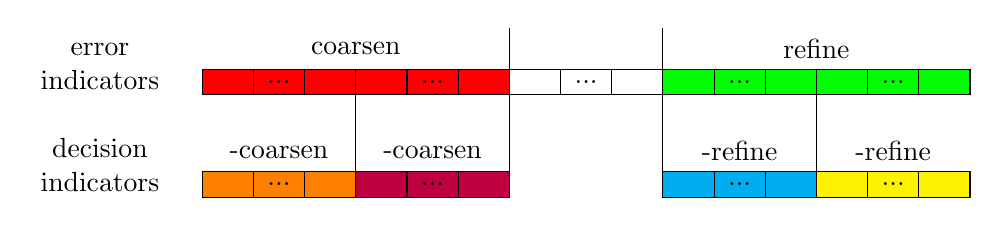
\begin{tikzpicture}[
  scale=0.65,
  valign/.style={%
    text height=1.5ex,
    text depth=.25ex,
  }
]

% error indicators
\node[align=center, text width = 1.6cm] at ( -2,0.55) {error indicators};

\node[align=center] at ( 3,.9) {coarsen};
\fill[color=red] (0,0) rectangle (6,0.5);
\node[align=center] at ( 12,.9) {refine};
\fill[color=green] (9,0) rectangle (15,0.5);

\draw (0,0) rectangle (15,0.5);
\foreach \x in {1,...,14}
  \draw (\x,0) -- (\x,0.5);
\foreach \x in {0,...,4}
  \node[align=center] at (3*\x+1.5,0.25) {...};

\draw (6,1.3) -- (6,-2);
\draw (9,1.3) -- (9,-2);


% decision indicators
\node[align=center, text width = 1.6cm] at ( -2,-1.37) {decision indicators};

% hp coarsen
\node[valign,align=center] at ( 1.5,-1.1) {\p-coarsen};
\fill[color=orange] (0,-2) rectangle (3,-1.5);
\node[valign,align=center] at ( 4.5,-1.1) {\h-coarsen};
\fill[color=purple] (3,-2) rectangle (6,-1.5);

\draw (0,-2) rectangle (6,-1.5);
\foreach \x in {1,...,5}
  \draw (\x,-2) -- (\x,-1.5);
\foreach \x in {0,...,1}
  \node[align=center] at (3*\x+1.5,-1.75) {...};

\draw (3,0) -- (3,-2);

% hp refine
\node[align=center] at (10.5,-1.1) {\h-refine};
\fill[color=cyan] (9,-2) rectangle (12,-1.5);
\node[align=center] at (13.5,-1.1) {\p-refine};
\fill[color=yellow] (12,-2) rectangle (15,-1.5);

\draw (9,-2) rectangle (15,-1.5);
\foreach \x in {10,...,14}
  \draw (\x,-2) -- (\x,-1.5);
\foreach \x in {3,...,4}
  \node[align=center] at (3*\x+1.5,-1.75) {...};

\draw (12,0) -- (12,-2);
\end{tikzpicture}%
\caption[Assignment of cells for \hp-adaptation with the \textit{fixed-number} strategy.]{Assignment of cells for \hp-adaptation with the \textit{fixed-number} strategy. Each cell's identifier and its indicator are stored in designated containers, whose entries are sorted in an ascending order of the indicators. Specified fractions of cells will be marked for adaptation. Large error indicators suggest refinement, while small ones imply coarsening. A large polynomial degree shall be assigned at a large decision indicator, while a fine grid resolution will be applied at a lower one.}
\label{fig:indicators}
\end{figure}

In practice, we need all predicted errors already for the initialization of this method. We provide them with an initial \h- or \p-adaptation of the mesh, by setting all predicted errors to $\eta_K^\text{pred} = 0$ or $\eta_K^\text{pred} = \infty$, respectively. We recommend to begin with an initial \h-refinement since its error predictor from Eq.~(\ref{eq:errorratio_h}) tends to be more reliable.

This strategy is useful for scenarios to generate a tailored mesh after a few refinement iterations, but lacks applicability for time dependent problems since the refinement history is also connected to the time evolution here. However, this method is well suited to determine the initial grid for initial values of time dependent problems iteratively.



\subsection{Smoothness estimation}
\label{ssec:smoothness}

According to Eq.~(\ref{eq:errorbound_hp}), we notice that \p-adaptation has the largest impact on the error if its corresponding solution is sufficiently regular. Thus, determining the smoothness of the finite element approximation presents a reasonable indicator to decide between \h- and \p-adaptation.

The basic idea to quantify smoothness involves the transformation of the finite element approximation into its spectral representation. In one dimension, we expand it into a series of $L_2$-orthogonal basis functions $(P_k)_{k\in\mathbb{N}_0}$ on an interval $I = [a,b]$ with:
\begin{align}
u_{hp}(x) &= \sum\limits_{k} c_k \, P_k(x) \,\text{,} && \forall k \in \mathbb{N}_0 \text{, } x \in I \,\text{,} \\
\langle P_k, P_l \rangle &= 0 \,\text{,} && \forall k,l \in \mathbb{N}_0 \text{: } k \neq l \,\text{,}
\end{align}
and identify the smoothness as the rate of decay of the expansion coefficients $c_n$. In multi-dimensional cases, we formulate the expansion in the multi-index notation with tuples $\tuple{k} = (k_1, \dots, k_\text{dim}) \in \mathbb{N}_0^\text{dim}$ on each cell $K$:
\begin{align}
u_{hp}(\vec{x}) &= \sum\limits_{k_1 \geq 0} \dots \sum\limits_{k_\text{dim} \geq 0} c_{k_1, \dots, k_{\text{dim}}} P_{k_1, \dots, k_{\text{dim}}}(\vec{x}) = \sum_{\tuple{k} \geq 0} c_\tuple{k} P_\tuple{k}(\vec{x}) \,\text{,}  & \forall \vec{x} \in K \,\text{,}
\end{align}
where we consider the multi-dimensional expansion as a product of basis functions for every coordinate direction:
\begin{align}
\label{eq:spectral_multi} P_{\tuple{k}}(\vec{x}) \equiv P_{k_1, \dots, k_{\text{dim}}}(\vec{x}) &\coloneqq P_{k_1}(x_1) \dots P_{k_\text{dim}}(x_\text{dim}) \,\text{.}
\end{align}

In the following, we will present two different ways to estimate its smoothness with this method, namely with Legendre and Fourier series expansions.

\textcite{mavriplis1994} was the first to attribute smoothness characteristics to the decay of coefficients from a Legendre series expansion. Legendre polynomials $P_k$ are solutions to the one-dimensional Legendre differential equation on the interval $I = [-1,1]$:
\begin{align}
\frac{\differential{}}{\differential{x}} \left(\left(1-x^{2}\right) \frac{\differential{}}{\differential{x}} P_k(x)\right)+ k \left(k+1\right) P_k(x)=0 \,\text{.}
\end{align}
They can be constructed with Rodrigues' formula and fulfill the orthogonality criterion
\begin{align}
P_k(x) &= \frac{1}{2^k k!} \frac{\differential{}^k}{\differential{x}^k} \left( \left(x^2 - 1\right)^k \right) \,\text{,} \\
\label{eq:legendre_orthogonal} \langle P_k, P_l\rangle &= \int\limits_K P_k(x) P_l(x) \differential{x} = \frac{2}{2 k+1} \delta_{k l} \,\text{.}
\end{align}
The first few Legendre polynomials are depicted in Fig.~\ref{fig:legendre}. \textcite{dealiilegendre}

\begin{figure}
\centering
\begin{tikzpicture}
\begin{axis}[
  cycle list/Dark2,
  scale=1.15,
  xlabel=$x$,
  ylabel=$P_k(x)$,
  grid=major,
  legend style={at={(0.5,1.02)}, anchor=south, /tikz/every even column/.append style={column sep=0.5cm}},
  legend columns=3,
  legend cell align=left]
\addplot+[samples=2, domain=-1:1] {1};
\addlegendentry{$P_0 = 1$};

\addplot+[samples=20, domain=-1:1] {0.5*(3*x^2-1)};
\addlegendentry{$P_2 = \frac{1}{2} \left( 3x^2 - 1 \right)$};

\addplot+[samples=60, domain=-1:1] {0.125*(35*x^4 - 30*x^2 + 3)};
\addlegendentry{$P_4 = \frac{1}{8} \left( 35x^4 - 30x^2 + 3 \right)$};

\addplot+[samples=2, domain=-1:1] {x};
\addlegendentry{$P_1 = x$};

\addplot+[samples=40, domain=-1:1] {0.5*(5*x^3 - 3*x)};
\addlegendentry{$P_3 = \frac{1}{2} \left( 5x^3 - 3x \right)$};

\addplot+[samples=80, domain=-1:1] {0.125*(63*x^5 - 70*x^3 + 15*x)};
\addlegendentry{$P_5 = \frac{1}{8} \left( 63x^5 - 70x^3 + 15x \right)$};
\end{axis}
\end{tikzpicture}
\caption{The first six Legendre polynomials.}
\label{fig:legendre}
\end{figure}

In the finite element context, all calculations happen on reference cells $\widehat{K} = [0,1]^\text{dim}$. Thus we need to construct a $L_2$-orthogonal basis on its domain. Furthermore, we require the multi-dimensional variant of Legendre polynomials from Eq.~(\ref{eq:spectral_multi}). These so designed functions similarly correspond to the orthogonality requirement from Eq.~(\ref{eq:legendre_orthogonal}) \textcite{dealiilegendre}:
\begin{align}
\widetilde{P}_\tuple{k}(\vec{x}) &\coloneqq 2^{\text{dim}/2} \, P_{k_1}(2x_1 - 1) \dots P_{k_\text{dim}}(2x_\text{dim} - 1) \,\text{,} \\
\left\langle \widetilde{P}_\tuple{k}, \widetilde{P}_\tuple{l} \right\rangle &= \left(\prod\limits_{j \in \tuple{k}} \frac{2}{2j+1}\right) \delta_{\tuple{k} \tuple{l}} \,\text{.}
\end{align}

Further, the calculation of expansion coefficients requires a mapping of the finite element approximation to the reference cell. This is performed via the transformation $\vec{x} = \mat{F}_K(\vec{\widehat{x}})$, which maps a point $\vec{\widehat{x}}$ from the reference cell $\widehat{K}$ to the actual cell $K$. We denote any function $\varphi$ mapped on the reference cell as $\varphi(\vec{x}) = \varphi(\mat{F}_K(\vec{\widehat{x}})) \equiv \widehat{\varphi}(\vec{\widehat{x}})$. \textcite{dealiimapping}

With these considerations, we will finally calculate the Legendre expansion coefficients as follows:
\begin{align}
c_\tuple{k} &=
\left(\prod\limits_{j \in \tuple{k}} \frac{2j+1}{2}\right) \int\limits_{K} u_\text{hp}(\vec{x}) \, \widetilde{P}_\tuple{k}(\mat{F}_K^{-1}(\vec{x})) \differential{\vec{x}} \\
&= \left(\prod\limits_{j \in \tuple{k}} \frac{2j+1}{2}\right) \int\limits_{\widehat{K}} \widehat{u}_\text{hp}(\vec{\widehat{x}}) \, \widetilde{P}_\tuple{k}(\vec{\widehat{x}}) \, \left|\det \mat{J}(\vec{\widehat{x}})\right| \differential{\vec{\widehat{x}}} \,\text{,}
\end{align}
with the determinant of the Jacobian $\mat{J}(\vec{\widehat{x}}) = \widehat{\nabla} \mat{F}_K (\vec{\widehat{x}})$ resulting from the coordinate transformation. \textcite{dealiilegendre}

For one-dimensional scenarios, \textcite{mavriplis1994} expanded the finite element approximation in a power series of Legendre polynomials up to the order $p_K$ of the assigned finite element on cell $K$. \textcites{houston2005}{eibner2007} generalized their approach by considering multi-dimensional Legendre polynomials:
\begin{align}
u_\text{hp} (\vec{x}) \simeq u_{\text{hp},\tuple{k}} (\vec{x}) &= \sum\limits_{0 \leq \|\tuple{k}\|_1 \leq p_K} c_\tuple{k} \, P_\tuple{k}(\mat{F}_K^{-1}(\vec{x})) \,\text{,} \quad \forall \vec{x} \in K \,\text{.}
\end{align}

\textcite[Prop.~2]{eibner2007} argued that a function is analytic, i.e.\@ representable by a power series, if and only if the absolute values of the expansion coefficients decay exponentially with an increasing index $\tuple{k}$:
\begin{align}
|c_\tuple{k}| \leq C \exp\left( - \sigma \|\tuple{k}\|_1\right) \,\text{,}
\end{align}
with constants $C$ and $\sigma > 0$. Thus a higher rate of decay $\sigma$ corresponds to a function that is more easily represented by lower order polynomials. \textcites[Sec.~2.4]{houston2005}[Ch.~4]{eibner2007} interpreted the rate of decay $\sigma$ as a measure for the local smoothness of the finite element approximation and determine it on each cell $K$ by performing a least squares fit on
\begin{align}
\ln \left( \max\limits_{\|\tuple{k}\|_1} |c_{\tuple{k},K}| \right) \sim C_K - \sigma_K \|\tuple{k}\|_1 \,\text{,} \quad \forall \tuple{k} \in \mathbb{N}_0^\text{dim} \text{: } 0 \leq \|\tuple{k}\|_1 \leq p_K
\end{align}
where we take the maximum value over all expansion coefficients $c_\tuple{k}$ that correspond to the same sum of elements $\|\tuple{k}\|_1$ of the multi-index tuple $\tuple{k}$. \textcite{mavriplis1994} considered a similar approach in one dimension, but only used the last four expansion coefficients for the fit.

\textcite{mavriplis1994, eibner2007} treated the rate of decay as a decision criterion for \hp-refinement by comparing it to a user-provided absolute threshold $\delta$: A decay rate larger than the threshold indicates a good resolution of the finite element basis functions and would entail \p-refinement, while a smaller rate would express a bad resolution and thus suggest \h-refinement. They considered a threshold of $\delta = 1$ as sufficient.

As an alternative strategy, \textcite{bangerth2009} proposed to use the coefficients of a Fourier series expansion to determine the rate of decay (see also \textcite{dealiistep-27}). We will use sinusoidal functions that form an orthogonal basis on the reference cell $\widehat{K} = [0,1]^\text{dim}$ as follows:
\begin{align}
P_\tuple{k}(\vec{x}) &= \exp\left(- i \, 2\pi \tuple{k} \cdot \vec{x}\right) \,\text{,} \\
\langle P_\tuple{k}, P_\tuple{l} \rangle &= \int\limits_{\widehat{K}} P_\tuple{k}(\vec{x}) \, P_\tuple{l}^\ast(\vec{x}) \differential{\vec{x}} = \delta_{\tuple{k} \tuple{l}} \,\text{.}
\end{align}
We present the real parts of the first few Fourier basis function in Fig.~\ref{fig:fourier}.

\begin{figure}
\centering
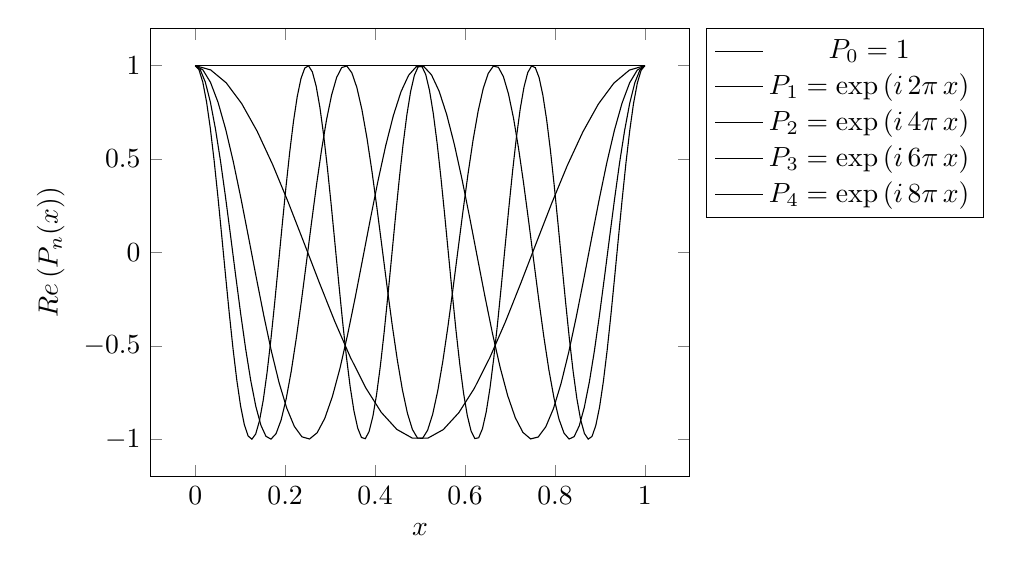
\begin{tikzpicture}
\begin{axis}[
  xlabel=$x$,
  ylabel=$\operatorname{Re}\left(P_n(x)\right)$,
  legend pos=outer north east]
\addplot[samples=2, domain=0:1] {1};
\addlegendentry{$P_0 = 1$};

\addplot[samples=30, domain=0:1] {cos(deg(6.28*x))};
\addlegendentry{$P_1 = \exp\left(i \, 2\pi \, x\right)$};

\addplot[samples=60, domain=0:1] {cos(deg(2*6.28*x))};
\addlegendentry{$P_2 = \exp\left(i \, 4\pi \, x\right)$};

\addplot[samples=90, domain=0:1] {cos(deg(3*6.28*x))};
\addlegendentry{$P_3 = \exp\left(i \, 6\pi \, x\right)$};

\addplot[samples=120, domain=0:1] {cos(deg(4*6.28*x))};
\addlegendentry{$P_4 = \exp\left(i \, 8\pi \, x\right)$};
\end{axis}
\end{tikzpicture}
\caption{The real parts of the first five basis functions of the Fourier expansion.}
\label{fig:fourier}
\end{figure}

Suppose our finite element approximation on cell $K$ is part of Hilbert space $H^s(K)$, the following integral must exist:
\begin{align}
\| \nabla^s u_{\text{hp}}(\vec{x}) \|_{L^2(K)}^2 = \int\limits_K \left| \nabla^s u_{\text{hp}}(\vec{x}) \right|^2 \differential{\vec{x}} < \infty \,\text{.}
\end{align}
The same condition also applies for its spectral representation $u_{\text{hp},\tuple{k}}$ and can be written as:
\begin{align}
\| \nabla^s u_{\text{hp}, \tuple{k}}(\vec{x}) \|_{L^2(K)}^2 &= \int\limits_K \left| \sum\limits_{\tuple{k}} (-i \, 2 \pi \tuple{k})^s \, c_\tuple{k} \, P_\tuple{k}(\mat{F}_K^{-1}(\vec{x})) \right|^2 \differential{\vec{x}} \\
&= (2 \pi)^{2s} \sum\limits_{\tuple{k}} \left| c_\tuple{k} \right|^2 \|\tuple{k}\|_2^{2s} < \infty \,\text{.}
\end{align}
The sum is finite only if we require that its summands decay as:
\begin{align}
\left| c_\tuple{k} \right|^2 \|\tuple{k}\|_2^{2s} \left\| \tuple{k} \right\|_2^{\text{dim} - 1} = \mathcal{O}\left( \|\tuple{k}\|_2^{-1-\epsilon} \right) \,\text{,} \quad \forall \epsilon > 0 \,\text{.}
\end{align}
The additional factor stems from the fact that, since we sum over all multi-indices $\tuple{k}$ that are located on a dim-dimensional sphere, we actually have, up to a constant, $\|\tuple{k}\|_2^{\text{dim}-1}$ modes located in each increment $\|\tuple{k}\|_2 + \differential{\|\tuple{k}\|_2}$ that need to be taken into account. \textcite{dealiistep-27}

With a comparison of exponents, we see that the Fourier coefficients must decay as follows so that the above integral exists:
\begin{align}
|c_\tuple{k}| = \mathcal{O}\left( \left\|\tuple{k}\right\|_2^{-\left(s + \frac{\text{dim}}{2} + \epsilon \right)} \right) \,\text{,} \quad \forall \epsilon > 0 \,\text{,}
\end{align}
or in other words, when the coefficients decay as $\left| c_\tuple{k} \right| = \mathcal{O}( \left\|\tuple{k}\right\|_2^{-\sigma-\epsilon} )$, then the finite element approximation $u_{hp}$ is part of $H^{\sigma - \text{dim}/2}$. \textcite{dealiistep-27}

We will expand the finite element approximation into a Fourier series on each cell $K$ and will use the local decay rate $\sigma_K$ of the expansion coefficients as a smoothness indicator. The basis functions of the spectral decomposition are complex-valued for Fourier expansions. Suppose our finite element approximation is real-valued, the expansion coefficients are symmetric $c_\tuple{k} = c_{-\tuple{k}}^*$ and we thus only have to calculate all positive multi-indices $\tuple{k}$. The expansion is performed as follows:
\begin{align}
u_{\text{hp}}(\vec{x}) &\simeq u_{\text{hp}, \tuple{k}}(\vec{x}) = \sum\limits_{0 \leq \|\tuple{k}\|_2 \leq p_K} c_\tuple{k} \, P_\tuple{k}(\mat{F}_K^{-1}(\vec{x})) \,\text{,} \\
c_\tuple{k} &=
\int\limits_K u_{\text{hp}}(\vec{x}) \, P_\tuple{k}^\ast(\mat{F}_K^{-1}(\vec{x})) \differential{\vec{x}} =
\int\limits_{\widehat{K}} \widehat{u}_{\text{hp}}(\vec{\widehat{x}}) \, P_\tuple{k}^\ast(\vec{\widehat{x}}) \, \left|\det \mat{J}(\vec{\widehat{x}})\right| \differential{\vec{\widehat{x}}} \,\text{.}
\end{align}
We expand our finite element approximation up to a mode that corresponds to the polynomial degree $p_K$ of the currently active finite element. From experience, we decided that this is a suitable choice. \textcite{dealiifourier}

With the expansion coefficients at hand, we calculate the decay rate with a least squares fit as follows:
\begin{align}
\ln\left( \max\limits_{\|\tuple{k}\|_2} c_{\tuple{k}, K} \right) \sim C_K - \sigma_K  \ln\left( \|\tuple{k}\|_2 \right) \,\text{,} \quad \forall \tuple{k} \in \mathbb{N}_0^\text{dim} \text{: } 0 < \|\tuple{k}\|_2 \leq p_K
\end{align}
We will skip the zeroth mode to avoid the singularity caused by the logarithm.

\textcite{bangerth2009} originally used these smoothness indicators as a decision criterion for \hp-refinement. They calculate the mean value of the smoothness indicator for all cells flagged for refinement. Whenever the indicator is larger than the average, \p-refinement is applied in favor of \h-refinement.

In our investigations, we will use both coefficient decay methods in separate scenarios to estimate the smoothness of our finite element approximation as decision criteria for \hp-adaptation. Further, we will expand them to utilize \hp-coarsening as well. For this, we will again use a strategy different from the ones presented by the original authors, namely the \textit{fixed-number} adaptation strategy. On cells to be refined, we consider the fraction corresponding to the largest decay rates for \p-adaptation, while for cells to be coarsened, the fraction with the lowest decay rates will be picked for \p-coarsening. This ensures the comparability of both methods.

In practice, we will calculate transformation matrices as auxiliary tools to convert a finite element approximation into its spectral representation. Thus we can perform the transformation by a simple matrix vector product. For every finite element in our collection, a separate transformation matrix has to be generated covering the number of modes corresponding to the polynomial degree $p$ of its basis functions.

For practical reasons, we will only create those matrices on the reference cell $\widehat{K} = [0,1]^\text{dim}$. This way we only have to perform the costly calculation of transformation matrices just once and will use them to determine the expansion coefficients on every cell $K$. On the downside, these transformations will only yield applicable results if the cells $K$ are not degenerate, or in other words, when mapping $\mat{F}_K$ from the reference cell $\widehat{K}$ to the actual cell $K$ is linear, resulting in a constant Jacobi determinant.

For the Legendre expansion, we determine the coefficients $c_{i,K}$ for each cell $K$ via matrix-vector product with the transformation matrix $\widehat{L}_{ij}$:
\begin{align}
&\forall \tuple{k} \in \mathbb{N}_0^\text{dim} \text{: } 0 \leq \|\tuple{k}\|_1 \leq p_K \,\text{,} &
c_{i(\tuple{k}),K} &= \sum\limits_j \widehat{L}_{i(\tuple{k})j} \, u_{j,K} \,\text{,} \\
&& \widehat{L}_{i(\tuple{k})j} &= \left(\prod\limits_{l \in \tuple{k}} \frac{2l+1}{2}\right) \int\limits_{\widehat{K}} \widehat{\phi}_j(\vec{\widehat{x}}) \, \widetilde{P}_\tuple{k}(\vec{\widehat{x}}) \differential{\vec{\widehat{x}}} \,\text{,}
\end{align}
where $u_{j,K}$ denote all entries of the solution vector belonging to the current cell $K$ and $\widehat{\phi}_j$ are the basis functions of the reference element. The map $i(\tuple{k})$ transforms the multi-index $\tuple{k}$ into an unique integer used as a matrix row index. When using Lagrange finite elements, we will use standard Gaussian quadrature to calculate the integrals with a number of quadrature points of $p_K + 1$ in each direction.

The rules to calculate the Fourier expansion coefficients $c_{i,K}$ with the corresponding transformation matrix $\widehat{F}_{ij}$ look slightly different:
\begin{align}
&\forall \tuple{k} \in \mathbb{N}_0^\text{dim} \text{: } 0 \leq \|\tuple{k}\|_2 \leq p_K \, \text{,} &
c_{i(\tuple{k}),K} &= \sum\limits_j \widehat{F}_{i(\tuple{k})j} \, u_{j,K} \,\text{,} \\
&& \widehat{F}_{i(\tuple{k})j} &= \int\limits_{\widehat{K}} \widehat{\phi}_j(\vec{\widehat{x}}) \, P_\tuple{k}^\ast(\vec{\widehat{x}}) \differential{\vec{\widehat{x}}} \,\text{.}
\end{align}
Since the Fourier basis function do not correspond to polynomials, but to sinusoids, we calculate the integrals differently. As a quadrature rule, we will iterate a base quadrature in each direction by a number of times corresponding to the highest mode, which we chose to be $p_K$. From our experience, a Gaussian quadrature with four points suffices for the role of the base rule.

In practice, we noticed that the coefficient decay strategies offer poor results on linear elements. We suspect that linear polynomials do not offer sufficient information to make a well-founded statement about the smoothness attribute of the finite element approximation on the cell itself. We thus suggest to refrain from using them in this context and work with at least quadratic elements instead.

A variety of different ideas and implementations for smoothness indication strategies have been elaborated in the past. \textcite{davydov2017} also used the method of Legendre coefficients, but determined their decay in each coordinate direction separately and took the minimum over all decay rates as the smoothness indicator. This approach ignores all multi-indices with more than one non-zero entry, which is why we do not consider this approach in our investigations.

A different approach is to estimate the Sobolev regularity locally and use it as a means for deciding between \h- and \p-adaptation. \textcite{ainsworth1998} presented a way to determine the regularity by solving the problem on smaller patches of the domain, which is rather expensive approach. On the other hand, \textcite{houston2003} proposed a strategy which estimates the local Sobolev regularity directly from a Legendre series expansion (see also \textcite[Sec.~2.4]{houston2005}). The latter method will form the basis of future enhancements on our \hp-adaptation strategies.

Further, we will investigate whether the determination of Fourier coefficients via \gls{fft} methods (e.g.\@ via \fftw{} \textcite{fftw338}) offers a more efficient and generally applicable alternative to the method presented above by \textcite{bangerth2009}.